\documentclass[a2paper, 12pt]{article}
\usepackage[font={huge, bf}]{caption}
\usepackage{fontspec}
\setmainfont{Arial}
\usepackage{subcaption}
\usepackage{graphicx}
\usepackage{tikz}
\usepackage{tikzsymbols}
\usetikzlibrary{calc,patterns,shapes.geometric}
\usepackage{float}
\usepackage{pdflscape}
\usepackage{geometry}
\geometry{landscape, margin=2cm}
\captionsetup[subfigure]{justification=justified,singlelinecheck=false}
\pagestyle{empty}

\def\centerarc[#1](#2)(#3:#4:#5){\draw[#1] ($(#2)+({#5*cos(#3)},{#5*sin(#3)})$) arc (#3:#4:#5);}

\begin{document}
	\vspace*{\fill}
	\begin{figure}[!htbp]
		\centering
		\begin{subfigure}[b]{0.48\textwidth}
			\caption{Figure 1}
			\centering
			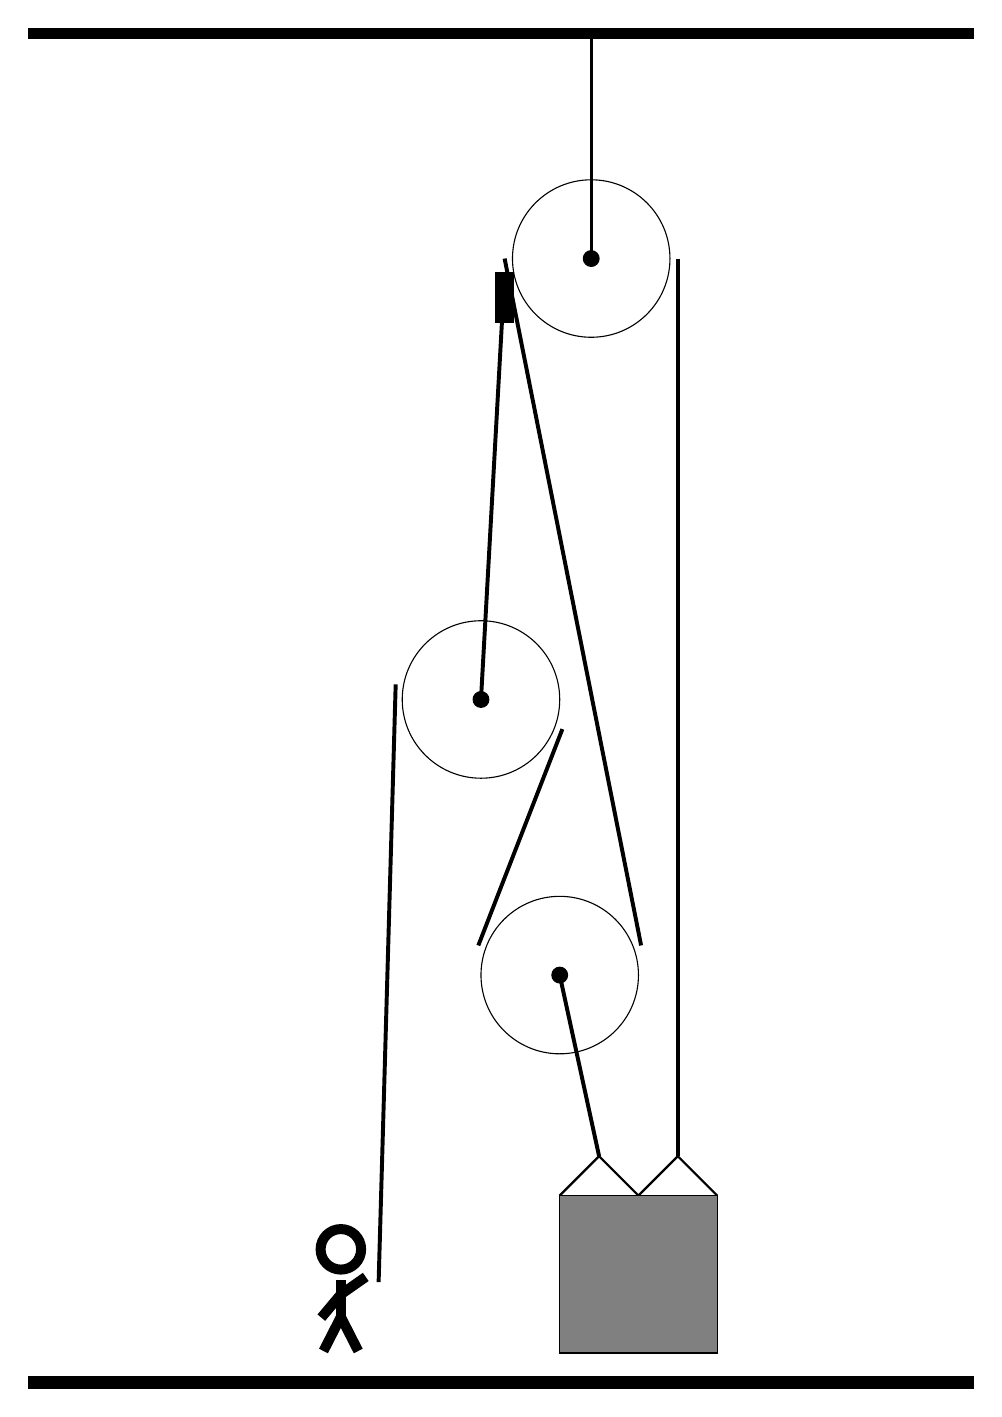
\begin{tikzpicture}
				\draw[fill=black] (-6, 14) rectangle (6, 14.125);
				
				\draw (-0.25, 5.6) circle (1);
				\draw[fill=black] (-0.25, 5.6) circle (0.1);
				
				\draw (0.75, 2.1) circle (1);
				\draw[fill=black] (0.75, 2.1) circle (0.1);
				
				\draw (1.15, 11.2) circle (1);
				\draw[fill=black] (1.15, 11.2) circle (0.1);
				\draw[very thick] (1.15, 11.2) -- (1.15, 14);
				
				\draw[thick]  (0.75, -0.7) -- (1.25, -0.2) -- (1.75, -0.7) -- (2.25, -0.2) -- (2.75, -0.7);
				\draw[fill=black!50] (0.75, -0.7) rectangle (2.75, -2.7);
				
				\draw[line width=0.5mm] (-0.25, 5.6) -- (0.05, 11.0);
				\draw[line width=0.5mm, fill=black](-0.05, 10.4) rectangle (0.15, 11.0);
				\draw[line width=0.5mm] (-1.55, -1.8) -- (-1.3333, 5.791);
				\centerarc[line width=0.5mm](-0.25, 5.6)(-20:170:1.1);
				\draw[line width=0.5mm] (0.7837, 5.2238) -- (-0.2837, 2.4762);
				\centerarc[line width=0.5mm](0.75, 2.1)(160:380:1.1);
				\draw[line width=0.5mm] (1.7837, 2.4762) -- (0.05, 11.2);
				\draw[line width=0.5mm](0.75, 2.1) -- (1.25, -0.2);
				\centerarc[line width=0.5mm](1.15, 11.2)(0:180:1.1);
				\draw[line width=0.5mm] (2.25, 11.2) -- (2.25, -0.2);
				
				\node at (-2, -1.9) {\scriptsize \Strichmaxerl[10][50][35]};
				
				\draw[fill=black] (-6, -3) rectangle (6, -3.15);
			\end{tikzpicture}
		\end{subfigure}
		\hfill
		\begin{subfigure}[b]{0.48\textwidth}
			\caption{Figure 2}
			\centering
			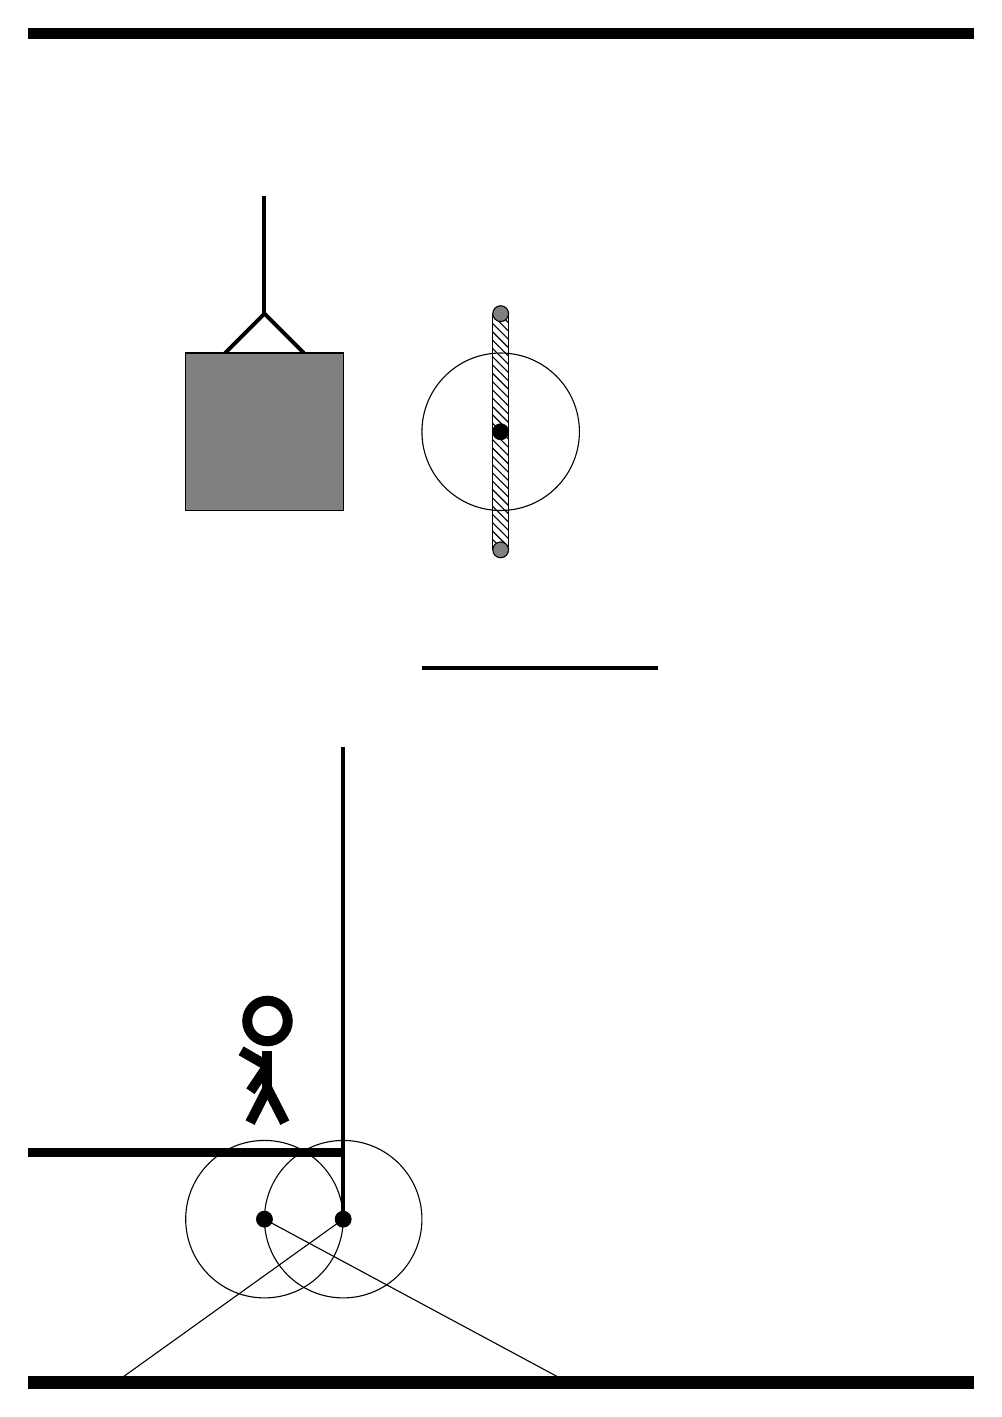
\begin{tikzpicture}
				\draw[fill=black] (-6, 14) rectangle (6, 14.125);
				
				\draw (0,9) circle (1);
				\draw[fill=black] (0,9) circle (0.1);
				\draw[pattern=north west lines, pattern color=black] (-0.1,10.5) rectangle (0.1,7.5);
				\draw[fill=black!50] (0,10.5) circle (0.1);
				\draw[fill=black!50] (0,7.5) circle (0.1);
				
				\draw (-2,-1) circle (1);
				\draw[fill=black] (-2,-1) circle (0.1);
				\draw (-5,-3.15) -- (-2,-1);
				
				\draw (-3,-1) circle (1);
				\draw[fill=black] (-3,-1) circle (0.1);
				\draw (1,-3.15) -- (-3,-1);
				
				\draw[line width=0.5mm](-3,10.5) -- (-3,12.0);
				\draw[line width=0.5mm](-3.5,10) --  (-3,10.5) -- (-2.5,10);
				\draw[fill=black!50] (-4, 10) rectangle (-2, 8);
				
				\draw[line width = 0.5mm] (-1,6) -- (2,6);
				\centerarc[line width = 0.5mm](-1,5)(90:180:1);
				\draw[line width = 0.5mm] (-2,5) -- (-2,-1);
				\centerarc[line width = 0.5mm](-1,-1)(180:360:1);
				
				\node at (-3, 1) {\scriptsize \Strichmaxerl[10][56][150]};
				\draw[fill=black] (-6, -0.10000000000000009) rectangle (-2, -0.19999999999999996);
				
				\draw[fill=black] (-6, -3) rectangle (6, -3.15);
			\end{tikzpicture}
		\end{subfigure}
	\end{figure}
		\vspace*{\fill}
\end{document}